%!TEX root = Report.tex
\begin{landscape}
\chapter{Estimated Models}\label{sec:models}

The models are described with the system matrices satisfying the following equation:
\[x(k + 1) = Ax(k) + Bu(k)\]
\[y(k) = Cx(k) + Du(k)\\\]
\\
where $x(k) \in \mathbb{R}^{7\times1}$, $u(k) \in \mathbb{R}$ and $y(k) \in \mathbb{R}$ for the FB case and $x(k) \in \mathbb{R}^{5\times1}$, $u(k) \in \mathbb{R}$ and $y(k) \in \mathbb{R}$\\ for the FF case.

The corresponding transfer functions $G(z) $ of both models are given as complex function in the frequency domain (z-Transform).

\section{Feedback}

System Matrices:
 
\[A = \left[ \begin{array}{ccccccc}

        0.9916  &   -0.3021  &  -0.01446  &   -0.3975  &    0.3342  &    0.8979   &   -1.751\\
    1.014\cdot10^{-5} &     0.9818   &   0.5898   &    0.189  &   -0.9155   &   -1.135   &    2.958\\
    -0.0006971 &   -0.02378  &     0.868   &   0.8622  &   -0.4149  &    -1.494   &    2.669\\
    0.0001233  &  0.002188   &  -0.1101  &    0.8439  &    -1.218  &   -0.9761    &   2.992\\
      0.0001113 &   0.001061 &   0.007756   &   0.1362  &    0.8197   &    1.692    &   -2.22\\
      9.92410^{-6} &  0.0001823 &   0.004315  &  -0.009561 &   -0.08712  &    0.8108   &   -2.475\\
     4.18110^{-7} & -1.14310^{-5} & -2.11210^{-5}  &  0.0001056 &  0.0008508  &   0.02776  &     1.011\\

\end{array} \right] \quad B = \left[ \begin{array}{c}

       -0.7629\\
      0.3258\\
       -0.08028\\
       -0.01179\\
      0.004377\\
      -0.00065\\
     -0.0001813\\

\end{array} \right]\] 

\[C =  \left[ \begin{array}{ccccccc}

   0.3142  &  0.472 &  -0.509 &   0.4186  & 0.3623 & -0.2782 &  -0.1635\\

\end{array} \right]  \quad D = 0\]

Transfer Function:
\[G(z) =\frac{-0.0482 z^{-1} + 0.2075 z^{-2} - 0.3771 z^{-3} + 0.3582 z^{-4} - 0.1727 z^{-5}+ 0.02859 z^{-6} + 0.003801 z^{-7}}{1 - 6.327 z^{-1} + 17.63 z^{-2} - 28.06 z^{-3} + 27.56 z^{-4} - 16.7 z^{-5} + 5.781 z^{-6} - 0.8801 z^{-7} }\] 

\section{Feedforward}

System Matrices:
 
\[A = \left[ \begin{array}{ccccc}

     0.9752   &   0.3421  &  -0.07598  &   -0.6669   &   0.8977 \\  
  -0.01128   &   0.9184    & -0.8166   &  -0.5002   &    1.722 \\
     0.000338 &     0.1704   &   0.8682  &     1.292   &   -1.428 \\
    0.001693  & -0.004514  &   -0.1086  &    0.8146   &   -2.106 \\
    -2.869\cdot10^{-5} &  -0.000823 &  -0.002818  &    0.0492  &    0.9329  \\

\end{array} \right] \quad B = \left[ \begin{array}{c}

        0.04258 \\
     -0.0002361\\
      -0.002666\\
      0.0002576\\
       0.000179\\

\end{array} \right]\] 

\[C =  \left[ \begin{array}{ccccccc}

   0.3763  & -0.4799 & -0.4982 &  0.4897 &   0.323\\

\end{array} \right]  \quad D = 0\\\]

Transfer Function:
\[G(z) =\frac{0.01765 z^{-1} - 0.06342 z^{-2} + 0.09233 z^{-3} - 0.0642 z^{-4} + 0.0181 z^{-5}}{ 1 - 4.509 z^{-1} + 8.509 z^{-2} - 8.402 z^{-3} + 4.338 z^{-4} - 0.9351 z^{-5} }\] 




\clearpage

\chapter{Singular Value Order Analysis}\label{sec:svd}

\section{Feedback Model}

\begin{figure}[H]
\centering
\begin{subfigure}[b]{0.38\textwidth}
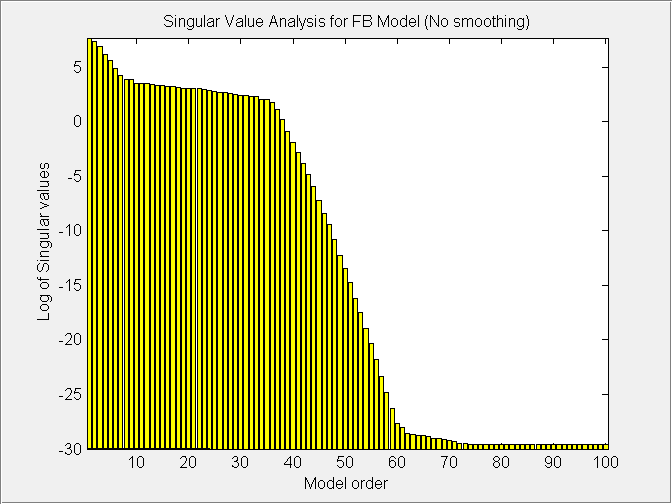
\includegraphics[width=1.0\textwidth]{pics/SVD_FB_inf}

\label{pic:}
\end{subfigure}\;\begin{subfigure}[b]{0.38\textwidth}
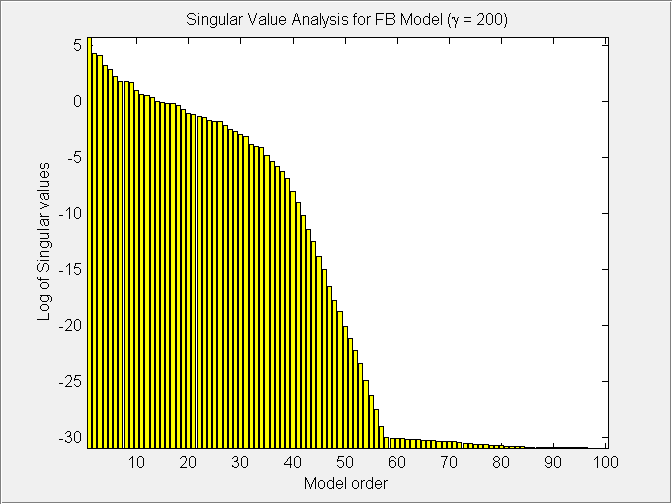
\includegraphics[width=1.0\textwidth]{pics/SVD_FB_200}

\label{pic:}
\end{subfigure}\;\begin{subfigure}[b]{0.38\textwidth}
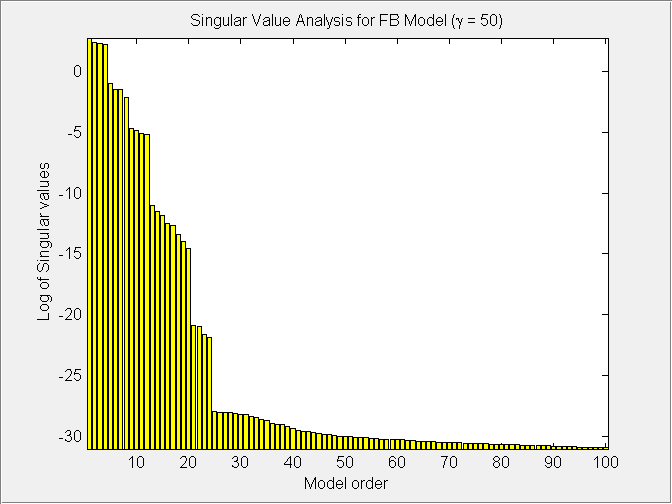
\includegraphics[width=1.0\textwidth]{pics/SVD_FB_50}

\label{pic:}
\end{subfigure}
\caption{Singular Value Order Analysis of Different Estimated Smoothed Empirical Transfer Functions (FB Model)}
\end{figure}

\section{Feed-forward Model}

\begin{figure}[H]
\centering
\begin{subfigure}[b]{0.38\textwidth}
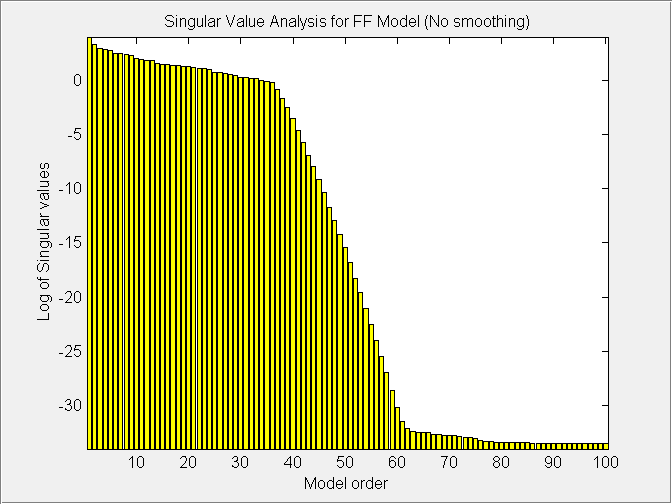
\includegraphics[width=1.0\textwidth]{pics/SVD_FF_inf}

\label{pic:}
\end{subfigure}\;\begin{subfigure}[b]{0.38\textwidth}
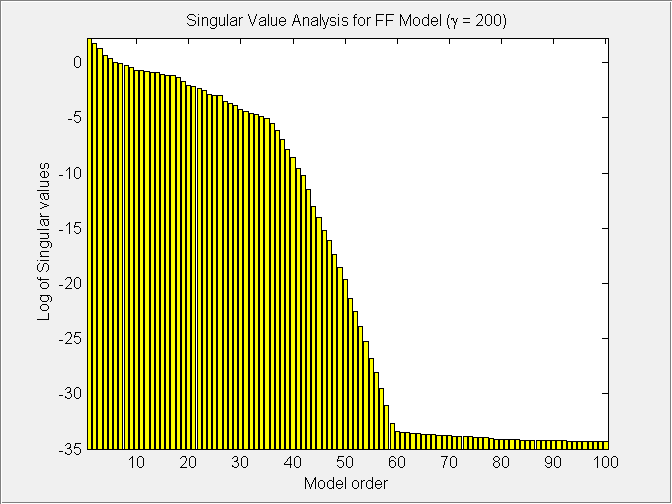
\includegraphics[width=1.0\textwidth]{pics/SVD_FF_200}

\label{pic:}
\end{subfigure}\;\begin{subfigure}[b]{0.38\textwidth}
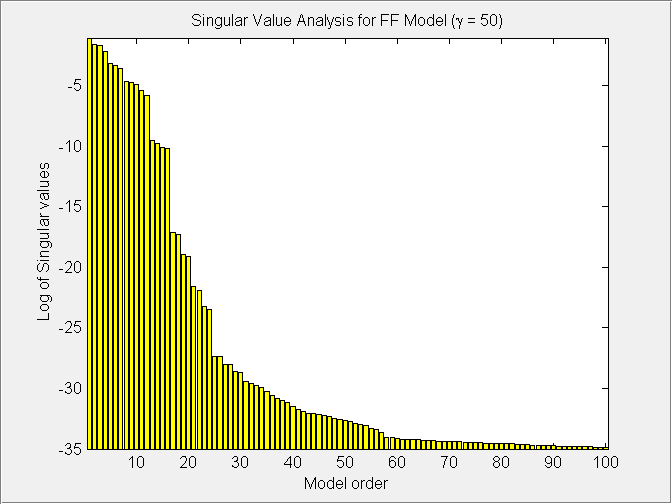
\includegraphics[width=1.0\textwidth]{pics/SVD_FF_50}

\label{pic:}
\end{subfigure}
\caption{Singular Value Order Analysis of Different Estimated Smoothed Empirical Transfer Functions (FF Model)}
\end{figure}

 \end{landscape}


\chapter{Parameter Optimization}\label{sec:RMS}

\section{Feedback Model}
\begin{figure}[h]
\centering
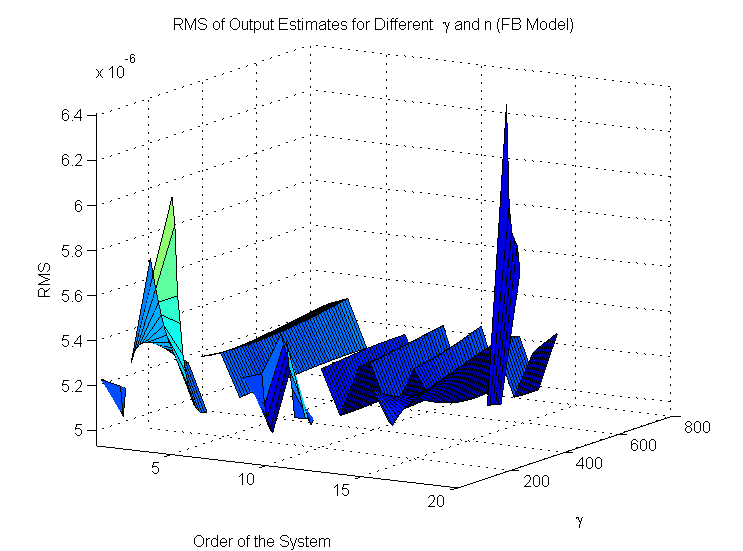
\includegraphics[width=0.6\textwidth]{pics/RMS_FB}
\caption{RMS of the Output Estimate Difference from Stable Feedback System Estimates Derived from Combinations of $\gamma$ and $n$}
\label{fig:RMS_FB}
\end{figure}

\section{Feed-forward Model}
\begin{figure}[h]
\centering
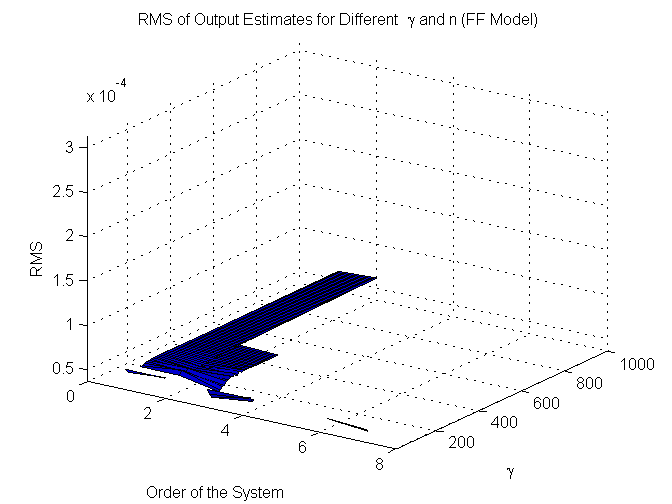
\includegraphics[width=0.6\textwidth]{pics/RMS_FF}
\caption{RMS of the Output Estimate Difference from Stable Feed-forward System Estimates Derived from Combinations of $\gamma$ and $n$}
\label{fig:RMS_FB}
\end{figure}











%\includepdf[pages=-,frame=true, scale=0.9]{pics/code.pdf}

%\includepdf[pages={1,3,4-5},angle=0,nup=2x2,frame=true, scale=0.9]{datasheets/PicDatasheet.pdf}
%\includepdf[pages=1]{datasheets/SharpDatasheet.pdf}
%
%\cleardoublepage

%
%\chapter{Something Else}\label{sec:something}
%
%Add here some other appendix material \dots
%
% \cleardoublepage
 
 

